\documentclass[12pt]{standalone}
\usepackage{tikz}

\begin{document}
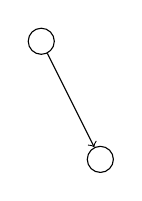
\begin{tikzpicture}
    \scoped[->,every node/.style={circle,draw}]
    \node (1){}
    child[missing] {}
    child {node(2) {}};
\end{tikzpicture}
\hskip 10pt
\begin{tikzpicture}
    \scoped[->,every node/.style={circle,draw}]
    \node (1){}
    child[missing] {}
    child {node(2) {}
            child[missing] {}
            child {node(3) {}}};
\end{tikzpicture}
\end{document}
